\documentclass{beamer}

\usepackage[T1]{fontenc}
\usepackage[utf8]{inputenc}
\usepackage[italian]{babel}
\usepackage{graphicx}
\usepackage{booktabs}
\usepackage{wrapfig}
\usepackage{xargs}
\usepackage{multicol}
\usepackage{minted}
\usepackage{csquotes}
\usepackage{verbatim}
%\usepackage[backend=biber,style=reading,sorting=none]{biblatex}

\mode<presentation> {
    \usetheme{Boadilla}
    \usecolortheme{beaver}
}

\title[Navigazione cognitiva in Alchemist]{
    Simulazione di evacuazione di folle in Alchemist: \\
    un modello di mappa mentale per pedoni cognitivi
}

\author{Lorenzo Paganelli}

\institute[]
{
    Alma Mater Studiorum $\cdot$ Università di Bologna\\
    Campus di Cesena%
}

\date{19 Marzo 2020}

\begin{document}

\begin{frame}
  \titlepage
\end{frame}

% Uncomment these lines for an automatically generated outline.
%\begin{frame}{Outline}
%  \tableofcontents
%\end{frame}

\definecolor{bostonuniversityred}{rgb}{0.8, 0.0, 0.0}

\begin{frame}{Eventi rilevanti}
\hfil\hfil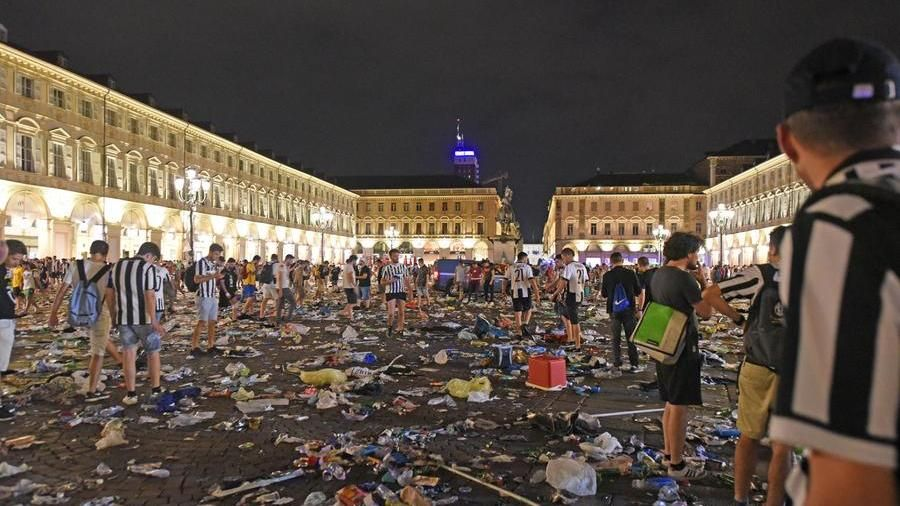
\includegraphics[width=5.5cm]{figures/piazza-san-carlo.jpeg}
\hfil\hfil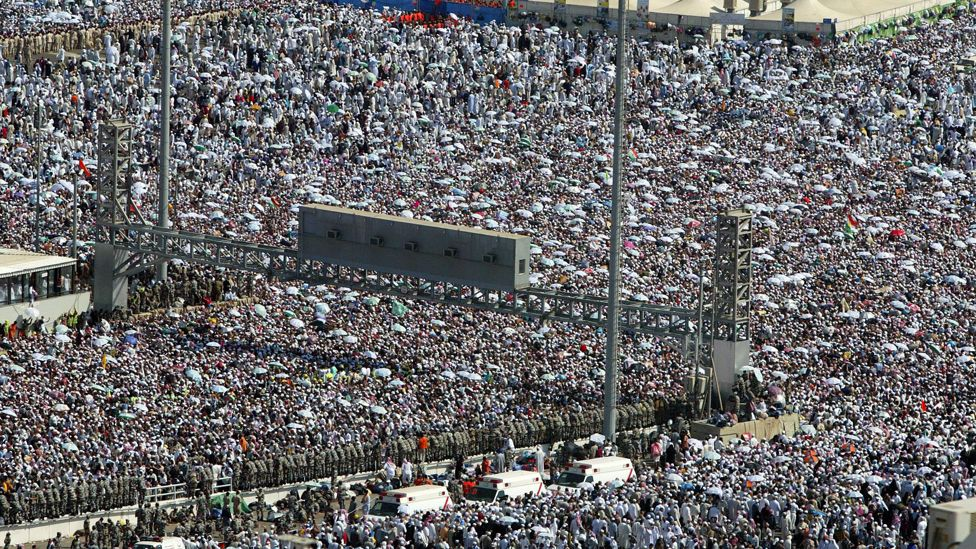
\includegraphics[width=5.5cm]{figures/hajj.jpg}
\newline
\null
\hfil\hfil\makebox[5.5cm]{Piazza San Carlo, Torino}
\hfil\hfil\makebox[5.5cm]{Ponte Jamarat, Mina}
\newline
\null
\hfil\hfil\makebox[5.5cm]{1500 feriti, 3 morti (2017)}
\hfil\hfil\makebox[5.5cm]{Più di 2000 morti (2015)}
\end{frame}

\begin{frame}{Simulazioni di evacuazione}
\hfil\hfil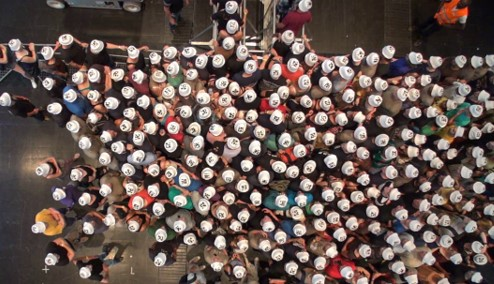
\includegraphics[width=5.5cm]{figures/real-simulation.jpg}
\hfil\hfil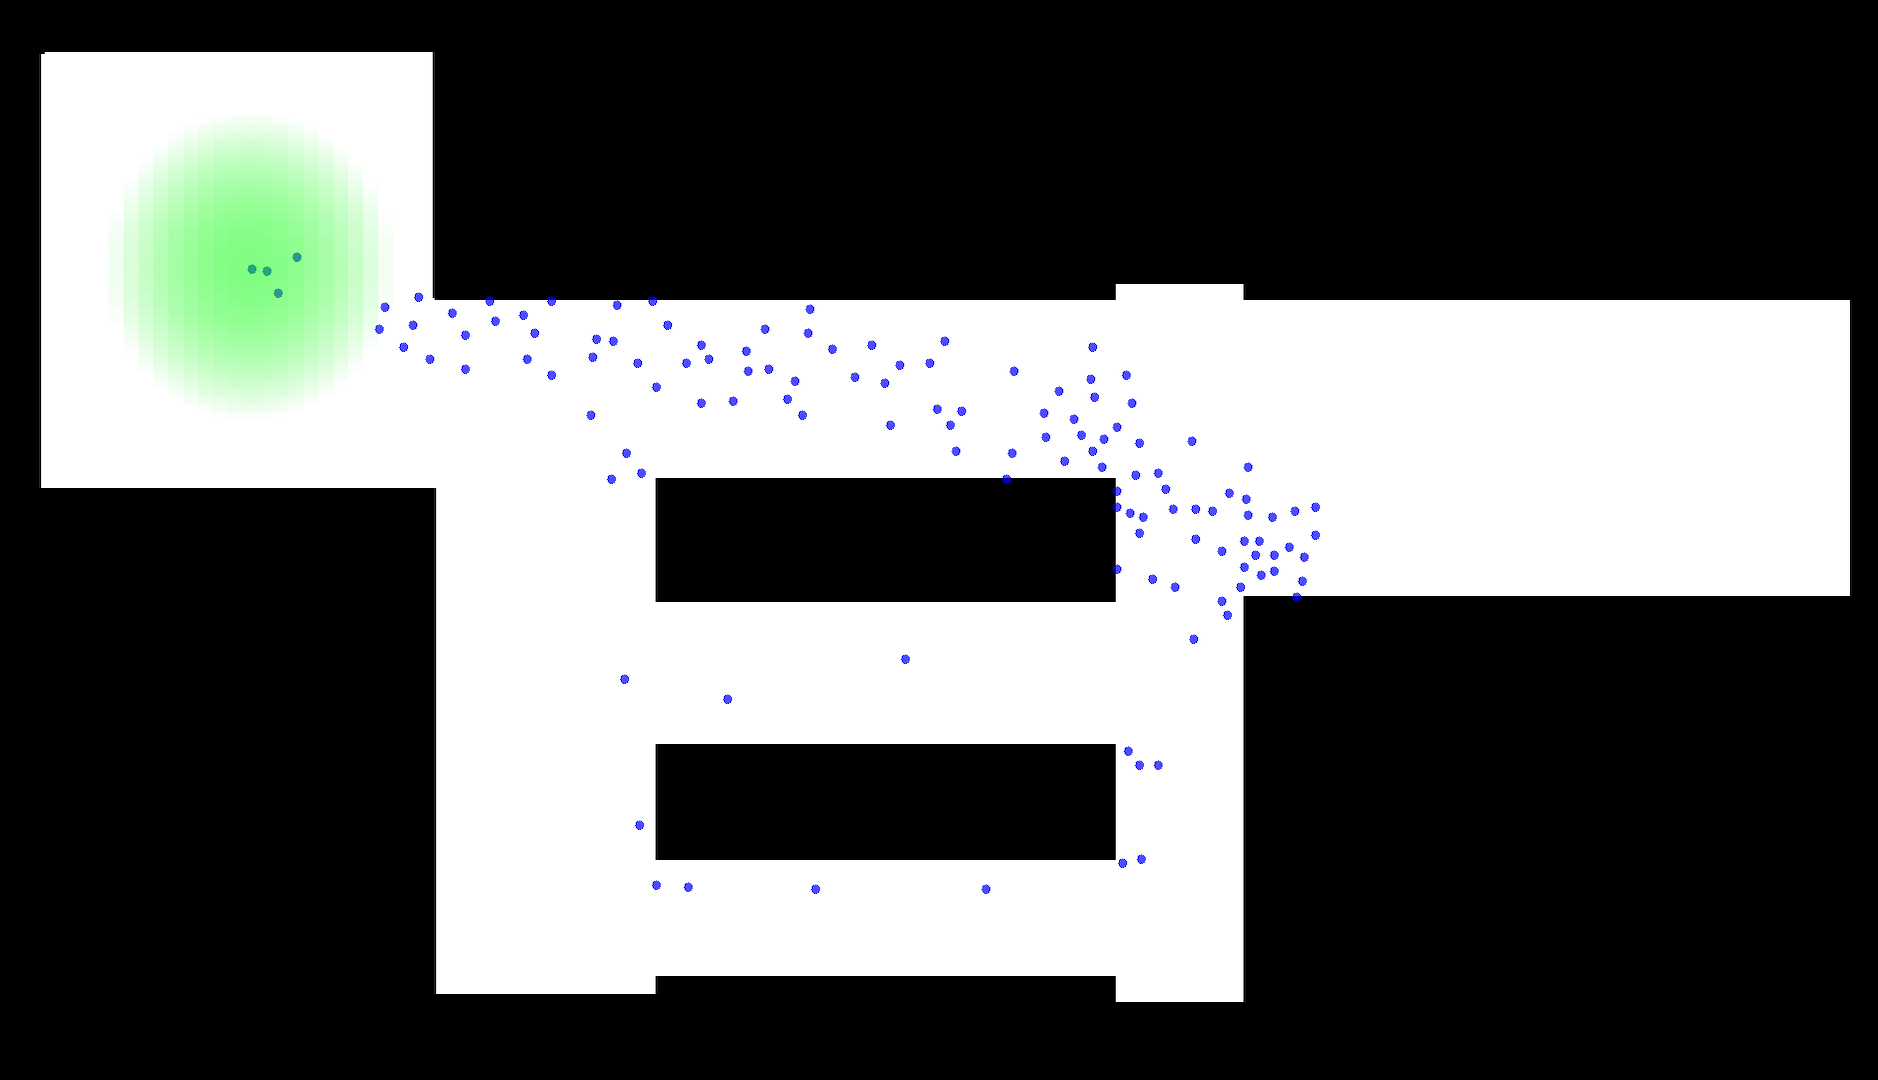
\includegraphics[width=5.5cm]{figures/computerised-simulation.png}
\newline
\null
\hfil\hfil\makebox[5.5cm]{Simulazione reale}
\hfil\hfil\makebox[5.5cm]{Simulazione computerizzata}
\end{frame}

\begin{frame}{Il simulatore Alchemist}
\begin{block}{Alchemist è}
Un simulatore nato all'interno dell'Università di Bologna che consente la simulazione di vari scenari, tra cui l'evacuazione di folle
\end{block}
\begin{block}{In Alchemist sono modellati}
Diversi aspetti psicologici e sociali dei pedoni
\end{block}
\begin{alertblock}{Problema}
I pedoni simulati in Alchemist sono sprovvisti della capacità di \textcolor{bostonuniversityred}{orientarsi}
\end{alertblock}
\end{frame}

\begin{frame}[fragile]{Pathfinding}
\hfil\hfil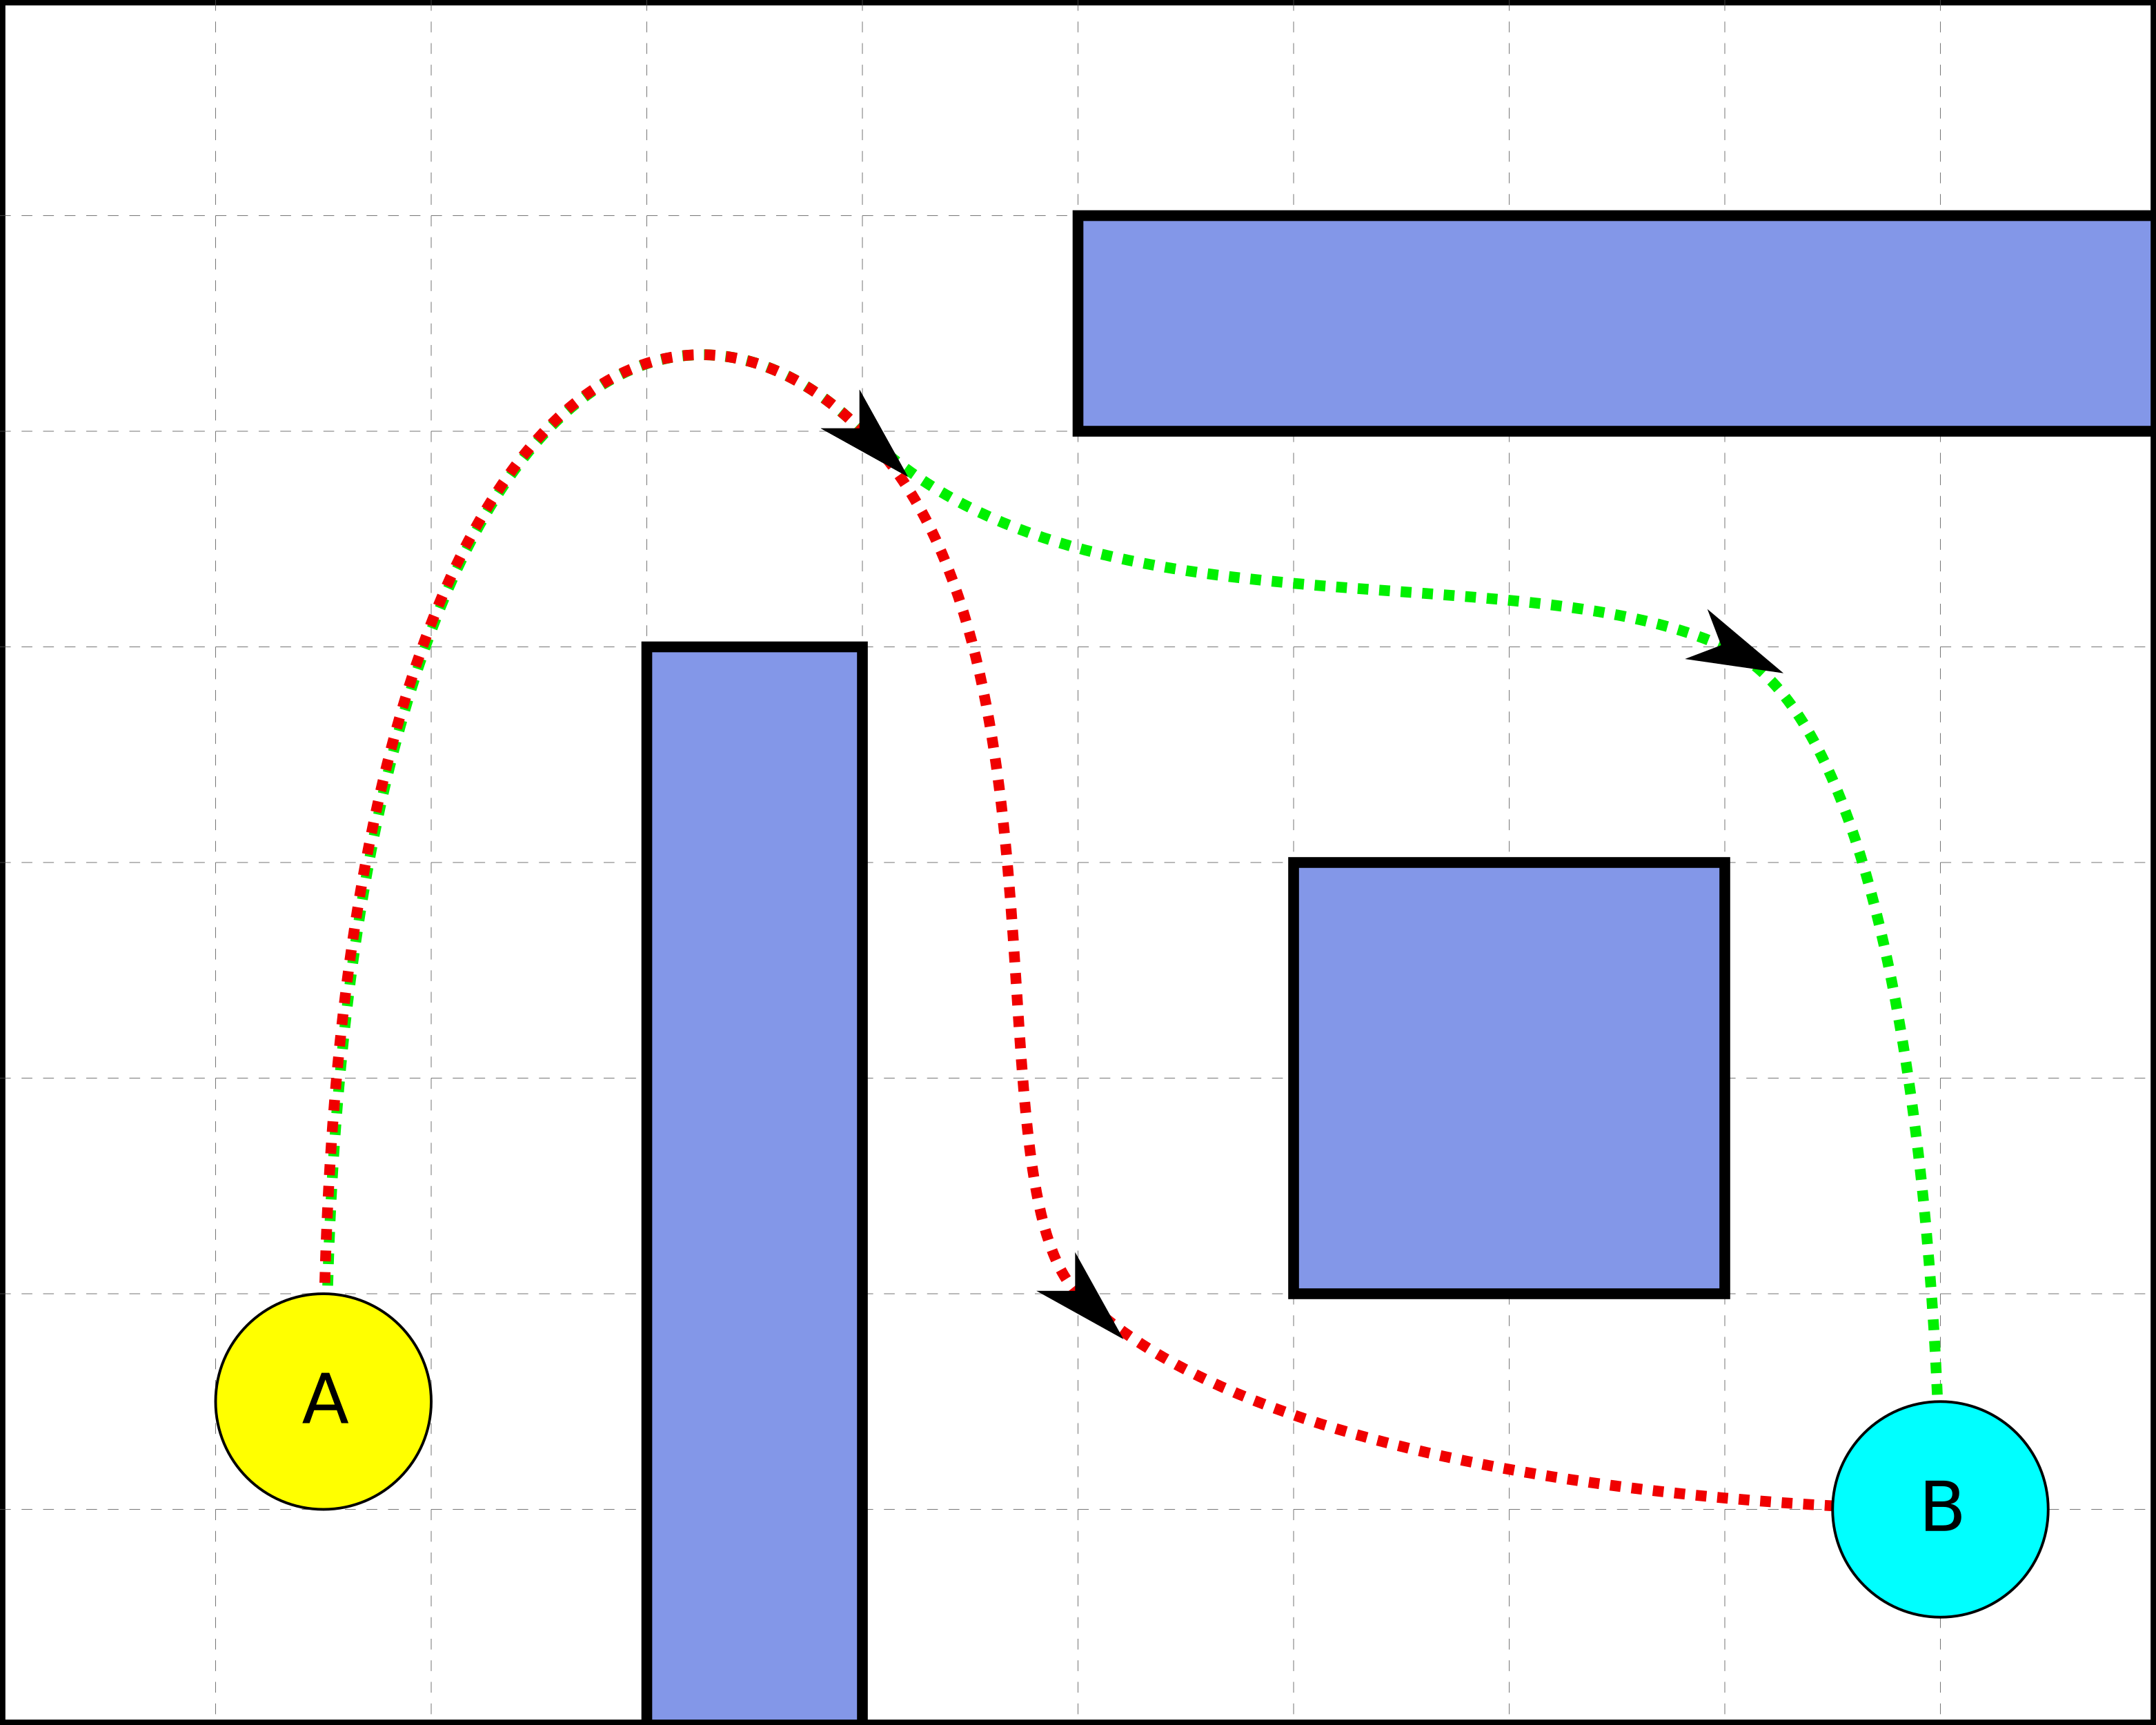
\includegraphics[width=9cm]{figures/pathfinding.png}
\end{frame}

\begin{frame}{Human wayfinding}
\begin{alertblock}{Problema}
Il pathfinding assume che i pedoni conoscano perfettamente l'ambiente, ma individui diversi hanno una \textcolor{bostonuniversityred}{conoscenza diversa} dello spazio circostante, spesso \textcolor{bostonuniversityred}{parziale} e \textcolor{bostonuniversityred}{inaccurata}
\end{alertblock}
\begin{block}{Obbiettivo}
Fornire i pedoni simulati di una tale eterogeneità
\end{block}
\end{frame}

\begin{frame}{Conoscenza spaziale}
\begin{block}{La mappa cognitiva è}
\begin{itemize}
    \item La rappresentazione mentale di un individuo dell’ambiente circostante
    \item Incompleta e inaccurata
\end{itemize}
\end{block}
\begin{alertblock}{Problema}
Che fare delle informazioni apprese dai pedoni durante la simulazione?
\end{alertblock}
\begin{block}{Soluzione: la memoria volatile}
\begin{itemize}
    \item Permette di riconoscere aree dell'ambiente già visitate durante l'evacuazione
    \item E' una mappa che ad ogni area associa il numero di visite
\end{itemize}{}
\end{block}{}
\end{frame}{}

\begin{frame}{Elaborazione di informazioni spaziali}
\begin{block}{Il sistema di pesi}
Assegna un peso \(w\) ad ogni arco \(e\) visibile, l'arco di peso minimo viene poi attraversato:
\begin{equation}
    w(e) = f_{volatile\ memory}\cdot f_{cognitive\ map}\cdot f_{final}\cdot \textcolor{bostonuniversityred}{f_{impasse}}\cdot \textcolor{bostonuniversityred}{f_{congestion}}
\end{equation}{}
\end{block}
\end{frame}

\begin{frame}{Esempi di simulazione}
\begin{block}{4 simulazioni}
\begin{itemize}
    \item Conoscenza completa
    \item Conoscenza parziale (30\%)
    \item Nessuna conoscenza
    \item Aggiramento delle congestioni
\end{itemize}
\end{block}
\end{frame}

\begin{frame}{Conclusioni e sviluppi futuri}
\begin{block}{In conclusione}
\begin{itemize}
    \item I pedoni realizzati presentano il comportamento desiderato
    \item I contributi fatti permettono di ottenere pattern di navigazione dell'ambiente più realistici
\end{itemize}{}
\end{block}
\begin{block}{Sviluppi futuri}
\begin{itemize}
    \item Raffinare quanto già presente
    \item Modellare caratteristiche e interazioni fisiche
\end{itemize}{}
\end{block}{}
\end{frame}{}

\begin{frame}{Riferimenti}
    \nocite{*}
    \bibliographystyle{plain}
    \bibliography{bibliography}
\end{frame}

\end{document}
